% path.png: the energy along the path of a jump, E(x) = a x^4 + b x^3 + c x^2. Make it in this folder with, for any scratch folder T:
%   pdflatex -output-directory=T fig_path.tex
%   python3 pdf_to_png.py T/fig_path.pdf ../path.png 1100
% Drawn for D = 1, Ks = 64 and dE = -1.2, hence a = 16, b = -4.8 and c = -7.595: minima at -0.3875 and 0.6125 with the energies -0.5004 and
% -1.7004 and the curvatures 24.8 and 39.2. The barrier 0.5004 is Ks D^2 / 64 (1 + 3u/4)^3 (1 - u/4) with u = 16 dE / (Ks D^2) = -0.3.
\documentclass[11pt,tikz,border=1.5pt]{standalone}
% Shared preamble of all figures. Every fig_*.tex is compiled on its own, see the comment at its top; the fonts are those of the matplotlib
% style xzc_sans (amsmath, amssymb, amsfonts, sfmath), so that line drawings and data plots look the same.
\usepackage{amsmath,amssymb,amsfonts}
\usepackage{sfmath}
\renewcommand{\familydefault}{\sfdefault}
\usepackage{graphicx}
\usetikzlibrary{arrows.meta,calc,positioning,decorations.pathreplacing,backgrounds,shapes.geometric}
% species: Al gray, Mg orange, Zn blue; red marks the vacancy and the jumping atom
\definecolor{cAl}{HTML}{B8BCC2}
\definecolor{cMg}{HTML}{E08A2E}
\definecolor{cZn}{HTML}{3F78B5}
\definecolor{cOne}{HTML}{C8423B}
\definecolor{cTwo}{HTML}{3F78B5}
\definecolor{cThree}{HTML}{3E9B5C}
\definecolor{cFour}{HTML}{E0A21B}
\definecolor{cGray}{HTML}{7E858F}
\definecolor{cDark}{HTML}{2B2B2B}
\newcommand{\panel}[1]{\textbf{(#1)}}
\newcommand{\DM}{D_{\mathrm{MEP}}}
\newcommand{\KI}{K_{\mathrm{I}}}
\newcommand{\KF}{K_{\mathrm{F}}}
\newcommand{\dE}{\Delta E}
\newcommand{\Ea}{\Delta E_{\mathrm{a}}}
\newcommand{\ea}{\Delta e_{\mathrm{a}}}
\newcommand{\Ebind}{E_{\mathrm{bind}}^{\mathrm{site}}}
% a ball with a soft highlight, like the rendered spheres
\makeatletter
\pgfdeclareradialshading[tikz@ball]{softball}{\pgfpoint{-9bp}{9bp}}{%
  color(0bp)=(tikz@ball!22!white); color(6bp)=(tikz@ball!62!white); color(13bp)=(tikz@ball!96!white);
  color(20bp)=(tikz@ball!92!black); color(27bp)=(tikz@ball!74!black); color(50bp)=(tikz@ball!55!black)}
\makeatother
\tikzset{
  every picture/.append style={line cap=round, line join=round},
  every node/.append style={font=\small},
  img/.style={inner sep=0pt, anchor=south west},
  lab/.style={font=\normalsize, inner sep=1pt, anchor=north west},
  above lab/.style={font=\normalsize, inner sep=1pt, anchor=south west},
  capt/.style={align=center, anchor=north},
  atom/.style={circle, ball color=#1, shading=softball, minimum size=12pt, inner sep=0pt},
  atom/.default=cAl,
  vac/.style={circle, draw=cOne, line width=1.1pt, fill=white, minimum size=11.5pt, inner sep=0pt},
  arr/.style={-{Stealth[length=5pt]}, line width=0.8pt},
  dbl/.style={{Stealth[length=4pt]}-{Stealth[length=4pt]}, line width=0.8pt},
  jump/.style={arr, cOne, line width=1.2pt},
  block/.style={-{Triangle[length=8pt, width=13pt]}, line width=5pt, cTwo!38},
  cell axis/.style={-{Triangle[length=6pt, width=5.5pt]}, line width=1.2pt, black},
  dir/.style={fill=white, fill opacity=0.75, text opacity=1, font=\footnotesize, inner sep=1.5pt},
}
\graphicspath{{img/}}
% data plots are included at one scale: \plot{name}{x}{y}{file}
\newcommand{\plotscale}{0.6}
\newcommand{\plot}[4]{\node[img] (#1) at (#2,#3) {\includegraphics[scale=\plotscale]{#4}};}
\newcommand{\plotlabel}[2]{\node[above lab] at ($(#1.north west)+(-0.05,0.02)$) {\panel{#2}};}
% legend of the species, first entry at (#1,#2): Al, Mg, Zn (and the vacancy)
\tikzset{leg/.style={anchor=base west, inner sep=2pt, yshift=-3.2pt}}
\newcommand{\specieslegend}[2]{%
  \foreach \lx/\lc/\lt in {0/cAl/Al, 1.2/cMg/Mg, 2.4/cZn/Zn} {
    \node[atom=\lc, minimum size=10pt] at ({#1+\lx},#2) {}; \node[leg] at ({#1+\lx+0.2},#2) {\lt};}}
\newcommand{\vacancylegend}[2]{\node[vac, minimum size=9.5pt] at (#1,#2) {}; \node[leg] at ({#1+0.2},#2) {vacancy};}

\begin{document}
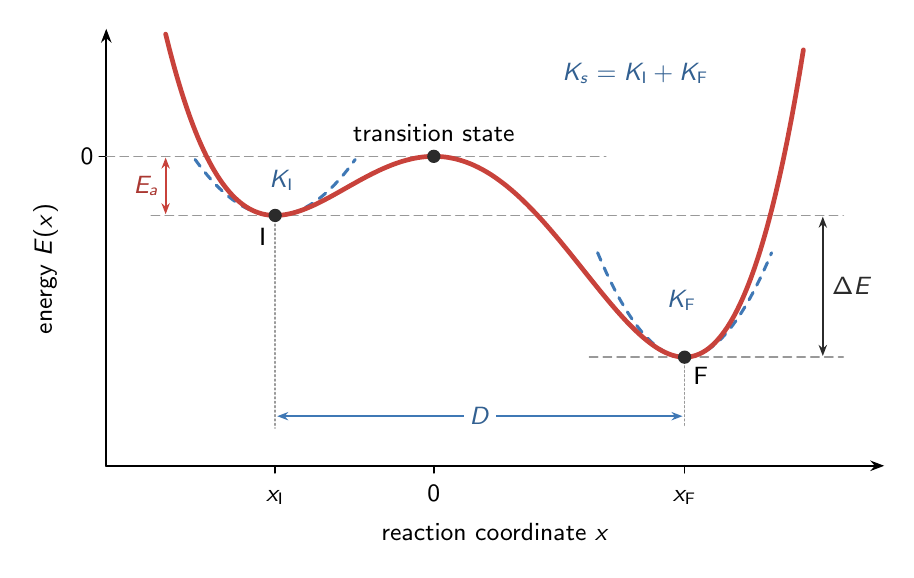
\begin{tikzpicture}[x=5.2cm, y=1.5cm]
  \draw[arr] (-0.80,-2.62) -- (1.10,-2.62) node[pos=0.5, below=17pt] {reaction coordinate $x$};
  \draw[arr] (-0.80,-2.62) -- (-0.80,1.08) node[pos=0.45, xshift=-15pt, rotate=90, anchor=south, inner sep=2pt] {energy $E(x)$};
  \foreach \x/\t in {-0.3875/x_{\mathrm{I}}, 0/0, 0.6125/x_{\mathrm{F}}} {
    \draw[line width=0.6pt] (\x,-2.62) -- ++(0,-0.06); \node[anchor=base, yshift=-13pt] at (\x,-2.62) {$\t$};}
  \draw[line width=0.6pt] (-0.80,0) -- ++(-0.017,0); \node[left, inner sep=3pt] at (-0.81,0) {$0$};
  % levels
  \draw[black!40, densely dashed, line width=0.6pt] (-0.80,0) -- (0.42,0) (-0.69,-0.5004) -- (1.0,-0.5004) (0.38,-1.7004) -- (1.0,-1.7004);
  \draw[black!40, densely dotted, line width=0.6pt] (-0.3875,-0.5004) -- (-0.3875,-2.30) (0.6125,-1.7004) -- (0.6125,-2.30);
  % parabolas with the curvatures at the two minima
  \draw[cTwo, dashed, line width=1.1pt] plot[domain=-0.583:-0.192, samples=40] (\x,{-0.5004 + 12.40*(\x+0.3875)^2});
  \draw[cTwo, dashed, line width=1.1pt] plot[domain=0.40:0.825, samples=40] (\x,{-1.7004 + 19.60*(\x-0.6125)^2});
  % the path
  \draw[cOne, line width=1.7pt] plot[smooth, domain=-0.655:0.905, samples=160] (\x,{16*(\x)^4 - 4.8*(\x)^3 - 7.595*(\x)^2});
  % barrier, energy change, distance
  \draw[dbl, cOne] (-0.655,-0.4904) -- (-0.655,-0.01) node[midway, left, inner sep=2pt, text=cOne!85!black] {$E_a$};
  \draw[dbl, cDark] (0.95,-0.5104) -- (0.95,-1.6904) node[midway, right, inner sep=3pt] {$\dE$};
  \draw[dbl, cTwo] (-0.3825,-2.20) -- (0.6075,-2.20) node[midway, fill=white, inner sep=2pt, text=cTwo!80!black] {$D$};
  \foreach \x/\y in {-0.3875/-0.5004, 0/0, 0.6125/-1.7004} \node[circle, fill=cDark, minimum size=4.8pt, inner sep=0pt] at (\x,\y) {};
  \node[above, inner sep=5pt] at (0,0) {transition state};
  \node[below left, inner sep=3pt] at (-0.3875,-0.53) {I};
  \node[below right, inner sep=3pt] at (0.6125,-1.71) {F};
  \node[text=cTwo!80!black] at (-0.372,-0.20) {$\KI$};
  \node[text=cTwo!80!black] at (0.605,-1.22) {$\KF$};
  \node[text=cTwo!80!black, anchor=west] at (0.29,0.70) {$K_s = \KI + \KF$};
\end{tikzpicture}
\end{document}
